\section{David Wineland}
\label{sec:Wineland}
The second half of the Nobel prize in physics 2012 was awarded to the American
quantum physicist David Wineland. David Wineland's work was driven by the will to
capture and take full control of single ions, leading for example to the
development of Doppler cooling. In this section we will first address
his early life and scientific career and then introduce important experimental
methods he established.

\subsection{Early Life and Scientific Career}
\begin{wrapfigure}{r}{0.34\textwidth}
  \centering
  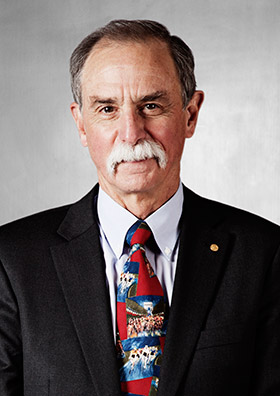
\includegraphics[width=.2\textwidth]{wineland.jpg}
  \caption{David Wineland in 2012.\\ Source: \textit{nobelprize.org}}
\end{wrapfigure}
David Wineland was born the same year as Serge Haroche on February 24, 1944,
in Wauwatosa, Wisconsin. His family moved to Sacramento, California in 1947
where he grew up and went to college. He describes his parents as marked by the
great depression emphasizing ``the importance of frugality and getting a good
education''~\cite{dwbio}. Having finished high school in 1961, Wineland enrolled
for a Math Major at the University of California. He soon realized that, working
hard enough, he could make it to the top of his class. Still in his junior year
he changed his university and subject and took up a Physics Major at Berkeley.
At the end of his undergraduate studies in physics he was not sure where to apply
for a Master and PhD, but asking his classical mechanics teacher helped a lot:
``he recommended Harvard, so I applied there''. This said he started his studies
at Harvard University in 1965 and soon joined the group of Norman Ramsey.\footnote{Nobel
prize in physics 1989 ``for the invention of the separated oscillatory fields
method and its use in the hydrogen maser''} 
There he got first in contact with experimental physics and decided to write his
PhD thesis about the hyperfine structure of deuterium~\cite{wineland1972atomic}.
In Ramsey's group, a working 
hydrogen maser had recently been accomplished and his goal was to realize similar
setups for all isotopes of hydrogen. After his PhD ended in  1970, Wineland
joined the group of Hans Dehmelt\footnote{Nobel prize in physics 1989 ``for the
development of the ion trap technique''.} who was at that time working on the
measurement of the anomalous magnetic moment of the electron. It became clear
that the most exact measurements would be performed on single trapped electrons,
so Wineland's goal was to trap a cloud of electrons and boil them out one by one
until only a single one would be left~\cite{wineland1973monoelectron}. During
that time he became hooked up on precision measurement and, having already
learned a lot about the trapping of charged particles, wanted to explore the
field of ion spectroscopy.

Looking for academic positions after his time as a postdoc he found one that
fully met his demands. The National Bureau of Standards (NBS, later National
Institute for Standards and Technology) was looking for somebody to join the
time and frequency domain and set up and calibrate a working cesium clock as a new time
standard. Within one year and a half, Wineland and his colleagues had calibrated
the clock to produce the new standard second. At that time there were plans for
the NBS to become more involved in basic research and consequently, in 1977,
Wineland got lab space and was joined by his first group members to work on
trapping and spectroscopy of ions. Up to today, he is the group leader of the
ion storage group at NIST with three of the four founding members still on
board. Their first goal was to demonstrate the
effect of laser cooling on trapped ions, an idea that had been proposed together
by Dehmelt and Wineland in 1975~\cite{wineland1975bullamphys}. They were under
quite some pressure as Wineland had heard from Dehmelt that he had taken a
sabbatical and joined the group of Peter Toschek in Heidelberg with the same
aim. Within only one year they had the first results and handed them in for
publication only one day apart from Dehmelt and
Toschek~\cite{wineland1978radiation, neuhauser1978optical}.\footnote{However
Dehmelt and Toschek beat them by one day.} Their experiment will
be discussed in Sec.~\ref{sec:DopplerCooling}. From that day on, Wineland and
his group continued to push the limits of single ion control for example by trapping
single ions in 1981~\cite{wineland1981spectroscopy}, demonstrating ion quantum
jumps in 1986~\cite{bergquist1986observation}, inventing the mechanism of resolved
sideband cooling in 1989~\cite{diedrich1989laser} or implementing the first quantum
logic gate in 1995~\cite{monroe1995demonstration}. Similar to the group of Serge
Haroche they found many applications of their methods to the fundamental
issues of quantum mechanics like many particle
entanglement~\cite{sackett2000experimental} or observation of the time evolution of
pure quantum mechanical states~\cite{leibfried2003quantum}.

In the following sections we will explore some of the methods and applications
developed by Wineland et al. in their chronic order. 


\subsection{Doppler Cooling}
\label{sec:DopplerCooling}

\begin{figure}[t]
  \centering
  \begin{subfigure}[t]{0.48\linewidth} 
    \centering
    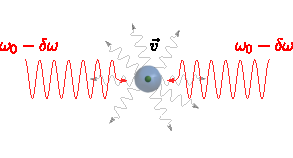
\includegraphics[width=\linewidth]{doppler_cooling_rep.pdf}
    \caption{The principle setup of Doppler cooling: two laser beams, red-detuned to a
    transition frequency of the atom $\omega_0$ shine in on the atom from opposite
  directions.}
    \label{fig:doppler_cooling}
  \end{subfigure}
  ~
  \begin{subfigure}[t]{0.48\linewidth} 
    \centering
    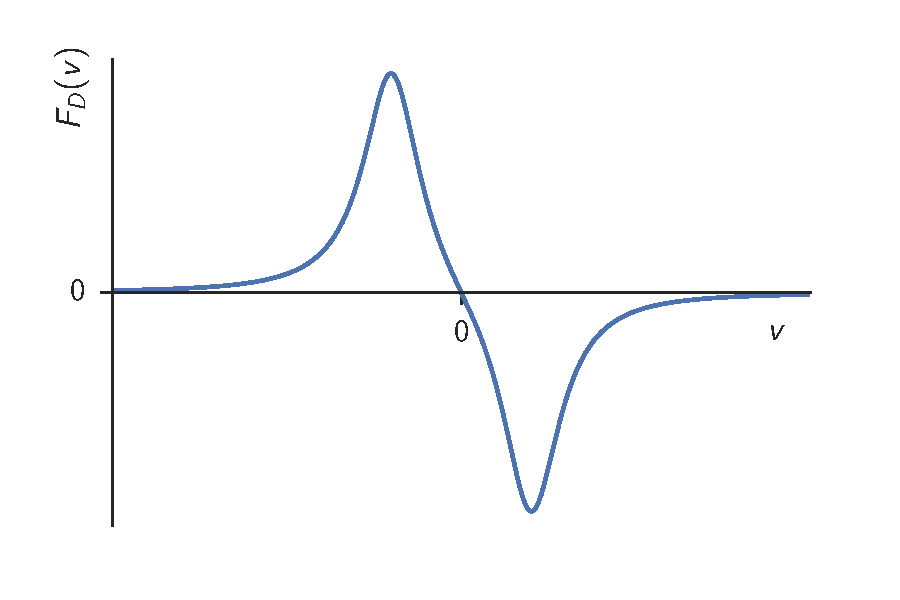
\includegraphics[width=\linewidth]{doppler_force.pdf}
    \caption{Force profile as a function of the velocity acting on an atom in a
    two-beam Doppler cooling configuration.}
    \label{fig:doppler_force}
  \end{subfigure}
  \caption{Principle of Doppler cooling and the resulting velocity dependent
  force profile.}
\end{figure}

The idea that atoms could be slowed down using a red-detuned laser was first
simultaneously proposed by Hans Dehmelt and David
Wineland~\cite{wineland1975bullamphys} and Theodor Hänsch and Arthur
Schawlow~\cite{hansch1975cooling} in 1975. Wineland and his group were the first
to publish experimental results that showed the desired
effect~\cite{wineland1978radiation} in 1978. The idea of Doppler cooling,
illustrated in Fig.~\ref{fig:doppler_cooling}, is the following: in a 1D setup
one shines two laser beams onto an atom from opposite directions. Both laser
beams are red-detuned by $\delta\omega$ with respect to a transition of the atom
$\omega_0$. If the atom now moves towards one of the beams, let's say with
velocity $+v$, it will be shifted
to resonance by the Doppler effect (thus the term Doppler cooling) and absorb
more photons from this direction, taking from each the momentum
$-\frac{\hbar\omega_0}{c}$. As the atom reemits the photons isotropically,
it will feel an overall force opposite to its direction of movement.
The force as a function of the velocity is given by
\begin{align}
  \label{eq:doppler_force}
  F_D(v) = \frac{\hbar \omega_0 I_{rel}}{2c\tau}\left[
  \frac{1}{1+\left(2\tau(\delta-v\omega_0/c)\right)^2}
-\frac{1}{1+\left(2\tau(\delta+v\omega_0/c)\right)^2}\right]
\end{align}
where $\tau$ is the lifetime of the state and $I_{rel}$ the light intensity
relative to the saturation intensity~\cite{mudrich2015}. The resulting force
profile is shown in Fig~\ref{fig:doppler_force}. We see that as long as the atom
moves around a velocity of $v=0$, it will experience a slow down force. We
note however that the Doppler force does not confine the atoms to a certain
position. For this one has to expand a setup by other features.

The setup that was used by Wineland et al. to demonstrate Doppler cooling is
shown in Fig~\ref{fig:cooling_setup}. A cloud of $^{24}$Mg$^{2+}$ ions is confined
in a Penning trap, made of two positive end caps, a negative ring electrode and a
magnetic field along the axis of the end caps.
\begin{figure}[t]
  \centering
  \begin{subfigure}[t]{0.48\linewidth} 
    \centering
    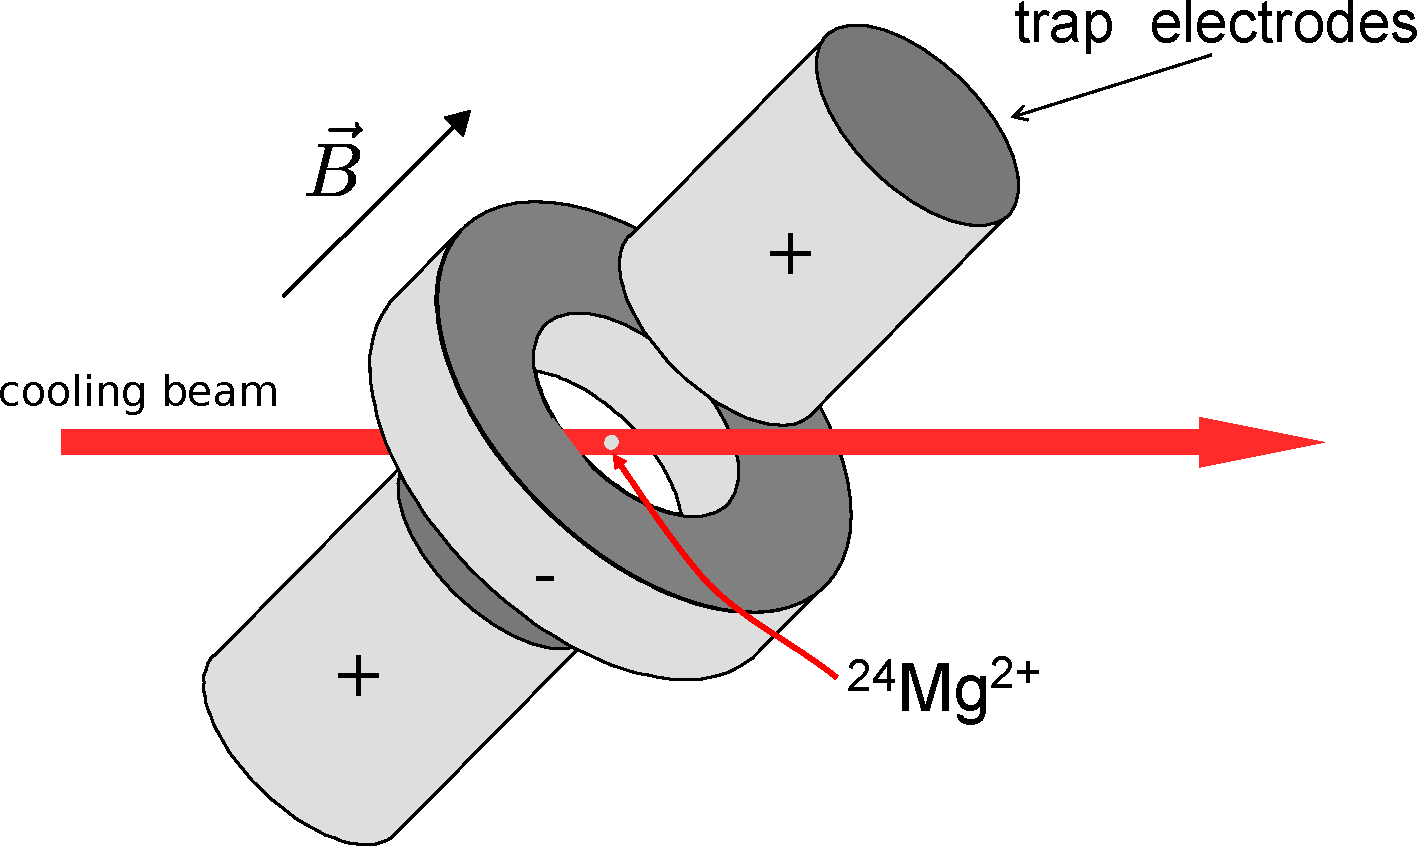
\includegraphics[width=\linewidth]{dw_laser_cooling_ions_setup.pdf}
    \caption{Setup used to Doppler cool a  cloud of magnesium ions. The ions are
    confined in a Penning trap with a red detuned laser beam going through
  the center of the trap.}
    \label{fig:cooling_setup}
  \end{subfigure}
  ~
  \begin{subfigure}[t]{0.48\linewidth} 
    \centering
    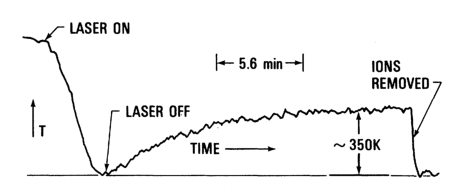
\includegraphics[width=\linewidth]{dw_laser_cooling_ions_plot.pdf}
    \caption{Ion temperature as a function of time. The ions were heated up
    before a cooling laser was switched on. After switching off the laser, the
  ions are allowed to rethermalize.}
    \label{fig:cooling_results}
  \end{subfigure}
  \caption{Setup used to cool down a cloud of magnesium ions and the resulting
    temperature evolution. (Sources: \cite{wineland2012nobel,wineland1978radiation})}
\end{figure}
A notable difference to the simplified scheme shown in
Fig~\ref{fig:doppler_cooling} is that there is only a single red-detuned laser
beam passing through the center of the trap. This is because the atoms are
confined in a harmonic trap. The laser beam is aligned with the axis of the
harmonic movement of the atoms in the trap, so any time the atoms move towards
the beam, they will be slowed down. In contrary to the free case, a second laser
is hence not necessary. The results of the experiment are shown in
Fig.~\ref{fig:cooling_results}. The signal that was recorded is the current
in the trap electrodes induced by the movement of the charged particles in the
trap and therefore proportional to $NT$ with $N$ being the number of particles
in the trap and $T$ their temperature. A significant particle loss during the
time of the experiment could be ruled out, and thus the signal is directly
proportional to the particles' temperature. The atoms were first heated up by
the cooling laser detuned to {\em higher} frequencies and then cooled down by
the same laser detuned to lower frequencies until they reached a minimum value
around \SI{40}{K}. The cooling laser was then switched off completely to allow
the atoms to rethermalize with their environment. The temperature curve clearly
shows the effectiveness of the laser cooling principle.

Cooling down clouds of ions was already a step towards measuring atomic spectra
more exactly as it would reduce the effects of Doppler broadening. The idea to
continue towards even higher precision was to isolate single ions as Wineland
had already done with electrons during his postdoc in the group of Hans Dehmelt.


\subsection{Trapping Single Ions}
The typical procedure to trap single particles is to first trap an ensemble of
particles and then apply a process by which the particles are kicked out of the
trap one by one until there is only a single one left. Wineland and his group
were first able to isolate single ions in a Penning trap in 1980, using 
$^{24}$Mg$^+$-ions. The experimental setup is similar to the one which
demonstrated
laser cooling shown in Fig.~\ref{fig:cooling_setup}. The laser beam is now
additionally aligned slightly off the trap center against the cyclotron movement
of the ions to cool down radial degrees of freedom as well. In order to reduce the
number of ions in the trap, a beam of $^{25}$Mg atoms was pointed towards the
$^{24}$Mg ions in the trap. Eventually the atoms and ions would undergo an
inelastic scattering process of the type
\begin{align}
  \label{eq:inel_scat}
  \,^{25}\text{Mg}\, + \,^{24}\text{Mg}^+ \,\longrightarrow\, ^{25}\text{Mg}^+ \,+
  \,^{24}\text{Mg},
\end{align}
exchanging one electron. The $^{25}$Mg ions, having a different cyclotron
frequency due to their higher mass, could then be selectively driven out of the
trap by radio frequency excitation and the $^{24}$Mg atoms, being neutral, are
no longer confined in the trap. The number of atoms is surveyed by measuring the
intensity of the emitted fluorescence light, which is again proportional to the
number of trapped ions. A resulting intensity vs time curve is shown in
Fig.~\ref{fig:dw_single_mg_plot_rep}. The last step in the fluorescence
intensity, around \SI{50}{\second} long, coincide with a single trapped ion.
\begin{figure}[t]
  \centering
  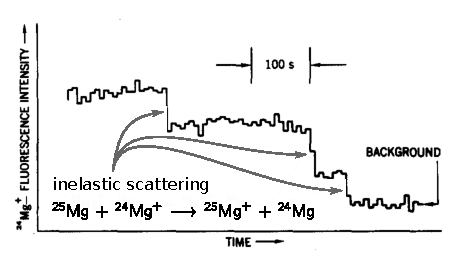
\includegraphics[width=0.7\linewidth]{dw_single_mg_plot_rep.pdf}
  \caption{Fluorescence intensity over time, as the ions are driven out of the
  trap by the indicated inelastic scattering process. The final step corresponds
  to only a single ion being left in the trap. (Adapted from
  \cite{wineland1981spectroscopy})}
  \label{fig:dw_single_mg_plot_rep}
\end{figure}

The ability to trap  single ions permitted many experiments that had until
then been impossible. All of the following experiments were only feasible with single
ions, as any interaction with other trapped ions would greatly perturb the
evolution of the ions' wavefunction.

\subsection{Ion Quantum Jumps}
Quantum jumps, the non-continuous transition of a quantum between its energy
states, are one of the most fundamental assumptions of quantum mechanics.
Nonetheless they have not been observed directly until the mid 1980s. Their
observation in ions necessitates a single ions as any ensemble effects would
smooth out the discreteness of appearing quantum jumps. David Wineland's group
was among the first to demonstrate quantum jumps in the internal energy state of a single
trapped ion in 1986~\cite{bergquist1986observation}. 
\begin{figure}[t]
  \centering
  \begin{subfigure}[t]{0.4\linewidth} 
    \centering
    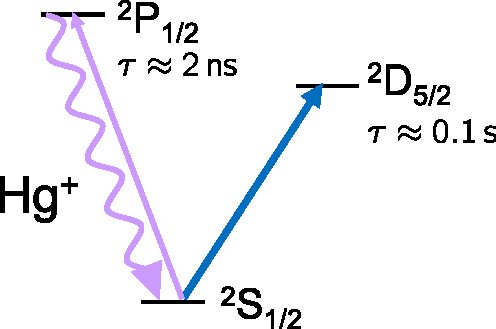
\includegraphics[width=.9\linewidth]{dw_quantum_jumps_level_scheme.pdf}
    \caption{Level scheme of Hg$^+$ used in the quantum jumps experiment. The
      S~$\rightarrow$~P transition is used for cooling and detection. The weaker
      S~$\rightarrow$~D is the ``quantum jump'' transition.}
    \label{fig:jumps_level_scheme}
  \end{subfigure}
  ~
  \begin{subfigure}[t]{0.48\linewidth} 
    \centering
    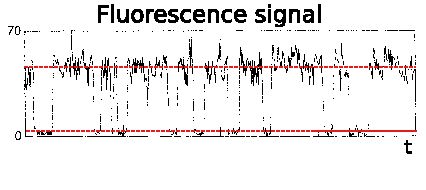
\includegraphics[width=\linewidth]{DW_quantum_jumps_results_rep.pdf}
    \caption{Fluorescence signal when both transitions are laser driven. The
    upper fluorescence level corresponds to the ion in the ground state, the
    lower one to the ion excited to the $^2$D$_{5/2}$ state.}
    \label{fig:jumps_results}
  \end{subfigure}
  \caption{Hg$^+$ level scheme and resulting fluorescence signal exhibiting
  jumps in the $^2$S$_{1/2}$ $\rightarrow$ $^2$D$_{5/2}$ transition. (Adapted
from \cite{wineland2012nobel} and \cite{bergquist1986observation})}
\end{figure}

The principle of quantum jump detection needs two transitions on different
timescales, like shown for the mercury ion in Fig.~\ref{fig:jumps_level_scheme}.
One transition, in this case $^2$S$_{1/2}$~$\rightarrow$~$^2$P$_{1/2}$ with
$\lambda_{S\rightarrow P} = \SI{194}{\nano\meter}$, is driven by a laser to cool
down the atom and record its fluorescence intensity. As long as the ion is in
the ground state, it will be constantly pumped to the $^2$P$_{1/2}$ state and
reemit a photon with an average rate of \SI{0.5}{\per\nano\second}. Additionally
a second much weaker transition, in this case the dipole forbidden
$^2$S$_{1/2}$~$\rightarrow$~$^2$D$_{5/2}$ with $\lambda_{S\rightarrow D} =
\SI{281}{\nano\meter}$, is driven by another laser. If the ion absorbs one of
the $\lambda_{S\rightarrow D}$ photons and ``jumps'' to the $^2$D$_{5/2}$ state,
the fluorescence on the first transition will suddenly stop, resulting in a
discrete step in the recorded fluorescence signal. As the lifetime of the weak
transition is much longer, one can in this way probe the state of the atom with
the rate of \SI{0.5}{\per\nano\second}.\footnote{In experiment the probing rate
is of course limited by the integration time of the intensity measurement.}
A resulting trace of the fluorescence signal is shown in
Fig.~\ref{fig:jumps_results}, showing sudden steps in the intensity that
correspond to jumps on the $^2$S$_{1/2}$~$\rightarrow$~$^2$D$_{5/2}$ transition.
This pattern is similar to the one observed by Serge Haroche in the case of
photons (Fig.~\ref{fig:quantum_jumps_results}) with the difference that the
weak transition is still much more frequent than the appearance of a single
photon.

In the same year also the group of Hans Dehmelt at Washington University and the
group of Peter Toschek in Heidelberg were able to show quantum jumps of a
trapped ion \cite{nagourney1986shelved, sauter1986observation}. Since then,
quantum jumps have also been observed for other systems like photons, electrons or
even molecules ~\cite{haroche2007QuantumJumps, gabrielse1992qnd,
basche1995direct}.

\subsection{Sideband Cooling}
Single ions could be Doppler cooled down to low temperatures, but the lowest
motional state in the trapping potential was still out of reach. This was about
to change with the resolution of motional sideband in trapped
ions~\cite{bergquist1987recoilless} in 1987 and the mechanism of resolved sideband
cooling in 1989~\cite{diedrich1989laser}. Wineland and his group realized that,
making use of the recoilless absorption of ions in a trap similar to the
Mössbauer effect and finely tunable lasers, they were able to cool down single
ions to their absolute motional ground state in an ion trap. As in the
quantum jump experiment they made use of the two transitions in the Hg$^+$ ion
depicted in Fig.~\ref{fig:jumps_level_scheme}, but this time the fluorescence
signal was recorded as the laser driving the S~$\rightarrow$~D was detuned by a
few \si{\mega\hertz} around resonance.
\begin{figure}[t]
  \centering
  \begin{subfigure}[t]{0.48\linewidth} 
    \centering
    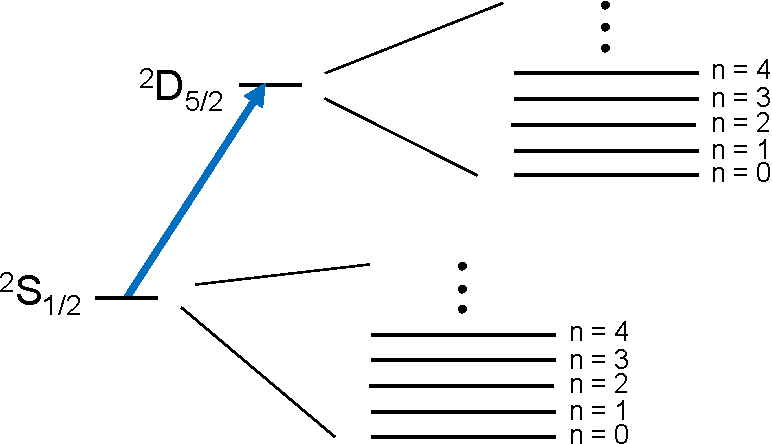
\includegraphics[width=\linewidth]{sideband_cooling_scheme_1_0_rep.pdf}
    \caption{Closeup of the level scheme of the trapped Hg$^+$ ion, including the motional
      splitting of the $^2$S$_{1/2}$ and the $^2$D$_{5/2}$ state in the trap.}
    \label{fig:motional_scheme1}
  \end{subfigure}
  ~
  \begin{subfigure}[t]{0.48\linewidth} 
    \centering
    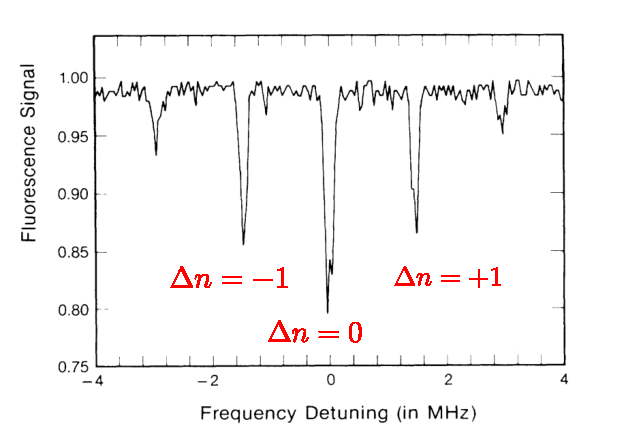
\includegraphics[width=\linewidth]{dw_quantized_motion_plot_rep.pdf}
    \caption{Intensity as a function of detuning of the S$\rightarrow$D laser.
    The discrete minima, reoccurring at fixed frequency intervals correspond to
  resonance between different motional levels.}
    \label{fig:quantized_motion_results}
  \end{subfigure}
  \caption{Scheme of quantized motional states of an ion in a trap and the
  resulting intensity signal. Again the fluorescence intensity of the
``probing'' transition S$\rightarrow$P was used to detect whether the ion is in
the ground or the metastable D state. (Adapted from
\cite{bergquist1987recoilless} and \cite{wineland2012nobel})}
\end{figure}
The resulting trace in Fig.~\ref{fig:quantized_motion_results} shows intensity
minima at a detuning of multiples of a frequency $\omega_{\text{trap}}$ around
resonance. That means that at this frequencies the ion is more likely to
undergo the S$\rightarrow$D transition. This behavior can be explained by
considering that the motional energy of an ion in a harmonic trapping potential
will be quantized, resulting in energy levels separated by
$\hbar\omega_{\text{trap}}$ were $\omega_{\text{trap}}$ is a characteristic
angular frequency. For $\omega_\text{trap}$ much smaller than the internal
resonance frequency $\omega_{S\rightarrow D}$ this will result in an energy level
in which any internal states will show sublevels corresponding to the motional
quantum $n$ like shown in Fig.~\ref{fig:motional_scheme1}.\footnote{This is in
  principal equivalent to the dressed states that appear in the treatment of the
  Jaynes-Cummings Hamiltonian (see Sec.~\ref{sec:DressedStates}) if we substitute the motional quantum $n$ by
the photon number $N$.}

How can a laser that resolves the motional levels of the trapped atom now be
used to cool the atom to its motional ground state? To explain this one first
needs to introduce the Lamb-Dicke regime, characterized by
\begin{align}
  \label{eq:lamb_dicke}
  \eta ^{2}(2n+1)\ll 1,
\end{align}
where $\eta$ is the Lamb-Dicke parameter and $n$ the motional quantum number.
Further $\eta$ is given by
\begin{align}
  \label{eq:def_eta}
  \eta^2 = \frac{\omega_R}{\omega_0},
\end{align}
where $\omega_0$ is the frequency of the laser, in our case driving the
S$\rightarrow$D transition, and $\omega_R$ corresponds to the recoil energy $E_R
= \hbar \omega_R = \frac{\hbar^2\omega_0^2}{2mc^2}$ that an atom gains upon
absorbing a photon of energy $\omega_0$. When $\eta^2$ and $n$ are both small,
i.e. when \eqref{eq:lamb_dicke} is fulfilled, the process of
spontaneous emission takes place on a different energy scale than the change of
the motional state. This means that in the Lamb-Dicke regime, the motional
quantum $n$ of a trapped ion will most likely not change upon spontaneous
emission of a photon.
\begin{figure}[t]
  \centering
  \begin{subfigure}[t]{0.33\linewidth}
    \centering
    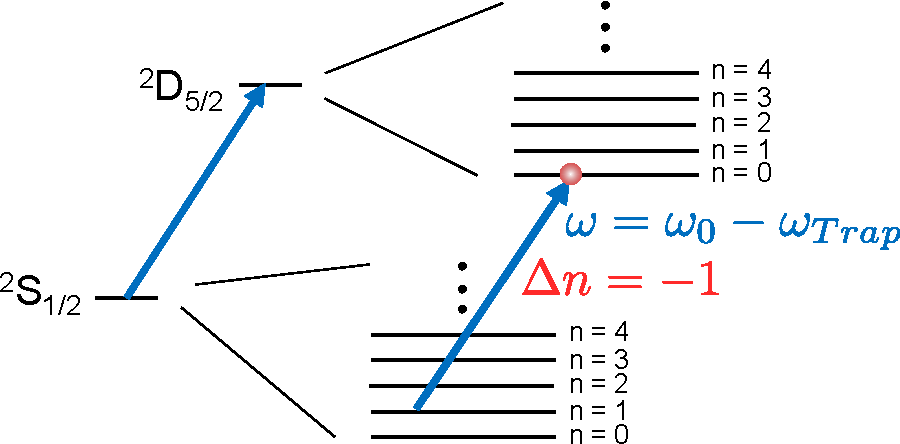
\includegraphics[width=\linewidth]{sideband_cooling_scheme_5_rep.pdf}
    \caption{The ion is excited on the blue motional sideband.}
  \end{subfigure}
  \begin{subfigure}[t]{0.3\linewidth}
    \centering
    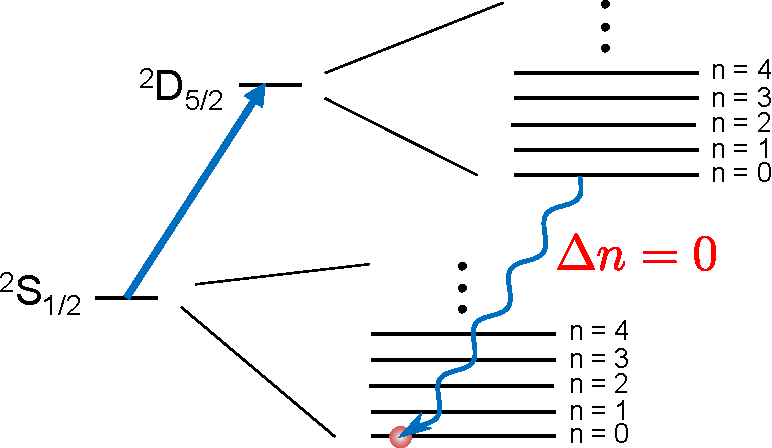
\includegraphics[width=\linewidth]{sideband_cooling_scheme_6_rep.pdf}
    \caption{The ion decays spontaneously without a change of $n$.}
  \end{subfigure}
  \begin{subfigure}[t]{0.3\linewidth}
    \centering
    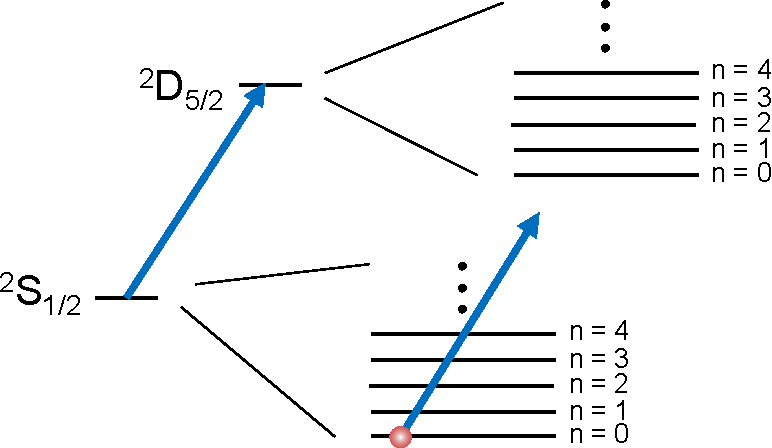
\includegraphics[width=\linewidth]{sideband_cooling_scheme_7_rep.pdf}
    \caption{The ion is in the lowest motional state and out of resonance with
    the laser.}
  \end{subfigure}
  \caption{One cycle of resolved sideband cooling, pumping the ion from $n=1$ to
  the lowest motional state $n=0$.}
  \label{fig:sideband_cooling}
\end{figure}
The described mechanisms can now be combined to the so called resolved sideband
cooling. The process is schematically shown in Fig.~\ref{fig:sideband_cooling}.
Assume the following setting: an ion is sitting in its internal ground state and
the motional state $n$ for which the Lamb-Dicke condition \eqref{eq:lamb_dicke}
is fulfilled. A laser is shone in on the red motional sideband frequency $\omega_0 -
\omega_\text{trap}$. The dynamics can then be described in three steps:
\begin{enumerate}[label=\alph*)]
  \item The ion absorbs one photon from the laser and will undergo the
    transmission from $\ket{g}\ket{n}$ to the excited state $\ket{e}\ket{n-1}$
    due to the red sideband condition.
  \item From the excited state $\ket{e}\ket{n-1}$ the ion will decay
    spontaneously to $\ket{g}\ket{n-1}$ without changing its motional state due to the Lamb-Dicke regime.
  \item The preceding two steps repeat until the ion is in the motional ground
    state of the trap $\ket{g}\ket{0}$ which is a dark state as there is no
    state $\ket{e}\ket{-1}$ fulfilling the resonance criterion.
\end{enumerate}

This procedure was first demonstrated to work by Wineland and his group in
1989~\cite{diedrich1989laser}. Cooling the ion to the motional ground state not
only increased the precision of frequency measurement, but was also the
foundation for later experiments in which full control of the motional and
internal states was needed. A good example for this is the implementation of a
quantum controlled-NOT gate, which will be discussed in the next section.

\subsection{Quantum Logic Gate}
Quantum computing has become a thriving field of theoretical physics,
experimental physics and cumputer sciences with even companies joining the search for
efficient and high fidelity implementations, since it was first proposed in
the 1980s by Feynman and others~\cite{feynman1982simulating}. The fundamental
difference to classical computing is that information is no longer stored in
classical bits that can be either 0 or 1 but in quantum bits (qubits) $\ket{0}$
and $\ket{1}$ that can occur in any superposition according to the
principles of quantum mechanics. This introduces new possibilities of coding,
e.g. Peter Shor proposed a qubit based algorithm to factorize integers in
polynomial time in 1994~\cite{shor1994algorithms}.\footnote{This discovery
triggered the new research field of post-quantum cryptography, as many current
cryptographic algorithms are based on the asymmetry of computational time
between multiplying two large prime numbers and factorizing the resulting
product. See for example~\cite{bernstein2009post}.} The implementation of
quantum algorithms requires the experimental realization of qubits and of
quantum logic gates, i.e. processes that perform basic logic operations on
qubits without destroying their quantum nature. In 1995 Wineland and his group
realized that both would be possible with cooled down, trapped single ions and
demonstrated the first working quantum logic gate, namely a controlled-NOT
gate~\cite{monroe1995demonstration}.

A controlled-NOT (CNOT) gate has two qubits of input: the control qubit and the
target qubit. Whenever the control qubit is $\ket{1}$, the target qubit is
flipped, when the control qubit is $\ket{0}$, the qubits remain unchanged. The
resulting operation on the four possible pure states of a system consisting  of two qubits
is shown in Fig.~\ref{fig:cnot_theory}.
\begin{figure}[t]
  \centering
  \begin{subfigure}[t]{0.48\linewidth} 
    \centering
    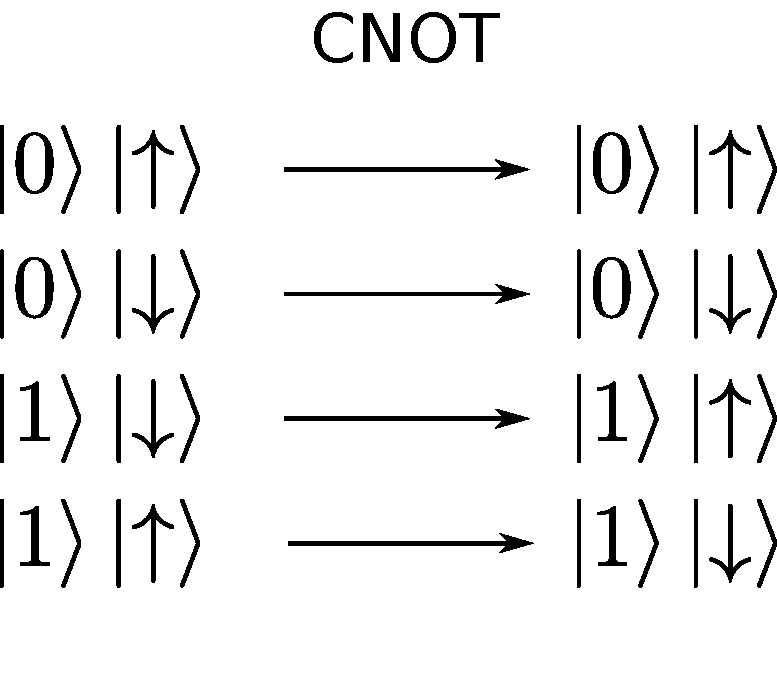
\includegraphics[width=.7\linewidth]{controled_not_rep.pdf}
    \caption{Theoretical action of a CNOT gate on the four possible pure states of a two
    qubit system. The first qubit acts as the control qubit, the second as the
  target qubit.}
    \label{fig:cnot_theory}
  \end{subfigure}
  ~
  \begin{subfigure}[t]{0.48\linewidth} 
    \centering
    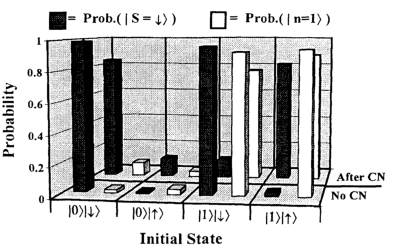
\includegraphics[width=\linewidth]{DW_cnot_gate_truthtable.pdf}
    \caption{Truth table of the experimentally realized CNOT gate. The white bars
    correspond to the motional qubit (control qubit), the black bars correspond
  to the internal qubit (target qubit).}
    \label{fig:cnot_experiment}
  \end{subfigure}
  \caption{Theoretical (a) and experimental (b) truth table of a quantum CNOT
  operation. (Adapted from \cite{monroe1995demonstration})}
\end{figure}
As Wineland's group was already able to control the motional and the internal
state of trapped ions, the idea was to use each of them to store one qubit of
information. Confining the ion to the lowest two motional states, the control
qubit would then be $\ket{n}$ with $n=0,1$. As long as any operation is shorter
than the lifetime of the internal state, the internal state being
$\ket{\uparrow}$ or $\ket{\downarrow}$ corresponding to the ion in the
excited or ground state, can be used as the target qubit. Experimentally these
states were the motional states of a trapped Ba$^+$ ion and its hyperfine states
$\ket{\uparrow} =\, ^2\text{S}_{1/2}\ket{F=2, m_f=2}$ and $\ket{\downarrow} =
\,^2\text{S}_{1/2}\ket{F=1, m_F=1}$. To implement the CNOT operation a third
auxiliary state $\ket{\text{aux}} = \,^2\text{S}_{1/2}\ket{F=2, m_F=0}$ was
used. The level scheme is shown in Fig.~\ref{fig:qubits_rep}. The four states
can be coupled by driving two off-resonant Raman beams (indicated by the
arrows). Depending on the difference frequency $\Delta$ between them, different states
are coupled. For $\Delta = \omega_0 + \omega_\text{trap}$ only
$\ket{0}\ket{\downarrow}$ and $\ket{1}\ket{\uparrow}$ are coupled. Shining in
with $\Delta = \omega_0 - \omega_\text{trap}$ will couple
$\ket{1}\ket{\downarrow}$ and $\ket{0}\ket{\uparrow}$. A detuning of $\Delta =
\omega_0$ will couple the upper and lower levels without changing the motional
quantum number. 
\begin{figure}[t]
  \centering
  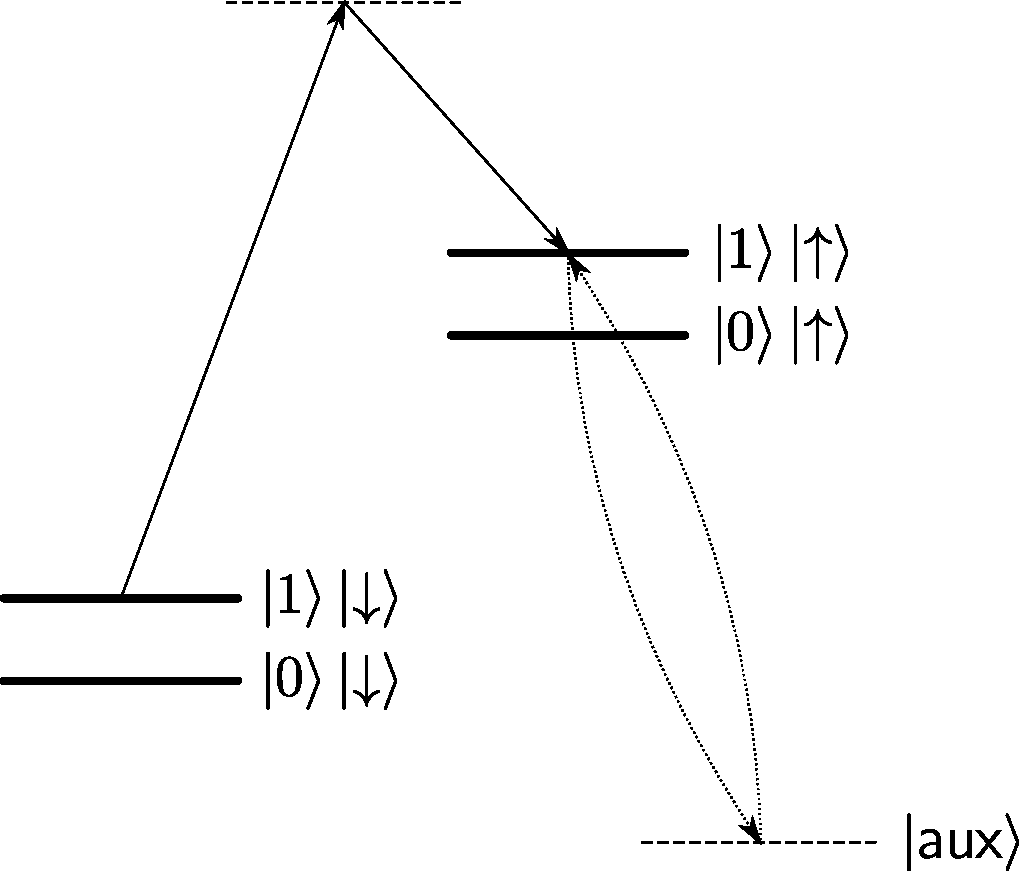
\includegraphics[width=0.4\linewidth]{qubits_rep.pdf}
  \caption{Level scheme of the two qubit system on which the CNOT operation was 
   implemented. Two Raman beams (solid arrows) can couple any pair of a lower 
   and an upper state, additionally $\ket{1}\ket{\uparrow}$ can be coupled to an 
 auxiliary level $\ket{\text{aux}}$ (dashed arrows).}
  \label{fig:qubits_rep}
\end{figure}

The implementation of the CNOT operation with the help of the three lasers
consists of a sequence of three Rabi pulses:
\begin{enumerate}
  \item A $\pi/2$-pulse of the Raman lasers with $\Delta=\omega_0$
  \item A 2$\pi$-pulse coupling $\ket{1}\ket{\uparrow}$ and $\ket{\text{aux}}$
  \item A $\pi/2$-pulse of the Raman lasers with $\Delta=\omega_0$ and a phase shift of $\pi$ relative
    to the first pulse
\end{enumerate}
To understand how this really defines a CNOT operation we go through the action
on a wave function step by step. The Rabi cycle shown in
Fig.~\ref{fig:rabi_cycle_rep} is of some help for illustration purposes. Assume
that the system is initially in the state
$$ \ket{\Psi_\text{init}} = \ket{1}\ket{\uparrow}.$$
In the first step this state is coupled to the lower lying $\ket{1}\ket{\downarrow}$ by a
$\pi/2$-pulse, taking it to the superposition state\footnote{Following the
nomenclature in Fig.~\ref{fig:rabi_cycle_rep} we identify
$\ket{1}\ket{\uparrow}$ with $\ket{e}$ and $\ket{1}\ket{\downarrow}$ with
$\ket{g}$.}
$$ \ket{\Psi_1} = \frac{1}{\sqrt{2}}\left(\ket{1}\ket{\uparrow}
-i\ket{1}\ket{\downarrow}\right)$$
The second step consists of applying a 2$\pi$-pulse on the auxiliary transition,
by which only the $\ket{1}\ket{\uparrow}$ part of the wavefunction will receive
a minus sign, resulting in
$$ \ket{\Psi_2} = -\frac{1}{\sqrt{2}}\left(\ket{1}\ket{\uparrow} + i
\ket{1}\ket{\downarrow}\right).$$
The last step is again a $\pi/2$-pulse on $\omega_0$ but shifted by $\pi$
relative to the first one, which corresponds to a counterclockwise step in
Fig.~\ref{fig:rabi_cycle_rep}, thus yielding
$$ \ket{\Psi_\text{final}} = -i\ket{1}\ket{\downarrow}$$
which will be detected as $\ket{1}\ket{\downarrow}$.\footnote{The detection
scheme of Wineland et al. in this case does explicitly not yield the full phase
information of the operation.} We see that in three steps
the target qubit has been flipped as expected for a control qubit of $\ket{1}$.
The other possible cases work accordingly, with any state with control qubit 
$\ket{0}$ being unaffected by the sign change in step 2 and thus not
experiencing a qubit flip.

The experimental results for prepared states before and after CNOT operation are
shown in Fig~\ref{fig:cnot_experiment}. It can be seen that the operation
qualitatively works as expected, interchanging the two states with control qubit
$\ket{1}$. Yet the fidelity is smaller than one due to effects of imperfect cooling or
decoherence. However the advantage of using ions as qubits is
that it can easily be scaled, for example by storing a larger number of ions in
a linear Paul trap using each of them to store two qubits of information. An
example of such an approach is the planned Q20:20 machine in Oxford, consisting
of twenty times twenty trapped ions that are optically linked to each
other\cite{walmsley2016}.
